% ============================================================
%  CV — Pierre Durocher · Software Engineer (preview example)
% ============================================================
\documentclass[9pt,a4paper]{extarticle}
\usepackage[T1]{fontenc}
\usepackage[utf8]{inputenc}
\usepackage[osf,sc]{mathpazo}
\usepackage{textcomp}
\usepackage{microtype}
\usepackage[a4paper,top=0.9cm,bottom=0.9cm,left=1.3cm,right=1.3cm]{geometry}
\usepackage{paracol}
\usepackage{enumitem}
\usepackage{graphicx}
\usepackage{xcolor}
\usepackage[hidelinks]{hyperref}
\usepackage{silence}
\WarningFilter{babel}{Command \showhyphens}
\pagestyle{empty}
\setlength{\parindent}{0pt}
\emergencystretch=1.5em
\hyphenpenalty=400
\providecommand{\up}[1]{\textsuperscript{#1}}
\newcommand{\lin}[1]{{\fontfamily{ppl}\selectfont #1}}
\definecolor{accent}{RGB}{39,76,175}
\newcommand{\cvsection}[1]{%
  \par\vspace{8pt}%
  {\noindent\color{accent}\large\scshape\textls[70]{#1}\par}%
  \vspace{1.5pt}{\noindent\color{accent}\rule{\linewidth}{0.5pt}\par}%
  \vspace{3.5pt}%
}
\newcommand{\cventry}[3]{%
  \par\vspace{5pt}\noindent
  {\bfseries #1}\hfill{\itshape\small #3}\par
  \vspace{0.5pt}\noindent{\small #2}\par
}
\newcommand{\cvlang}[2]{\noindent #1\hfill{\itshape #2}\par\vspace{2pt}}
\newcommand{\cvdomain}[2]{%
  {\small\bfseries\raggedright\hyphenpenalty=10000 #1\par}\vspace{1.5pt}%
  {\footnotesize\raggedright #2\par}}
\setlist[itemize]{label=\raisebox{0.22ex}{\scriptsize$\bullet$},
  leftmargin=1.1em, itemsep=1.2pt, topsep=3pt, parsep=0pt, partopsep=0pt}

\begin{document}

% ---------- HEADER ----------
\noindent
\begin{minipage}[c]{2.6cm}
  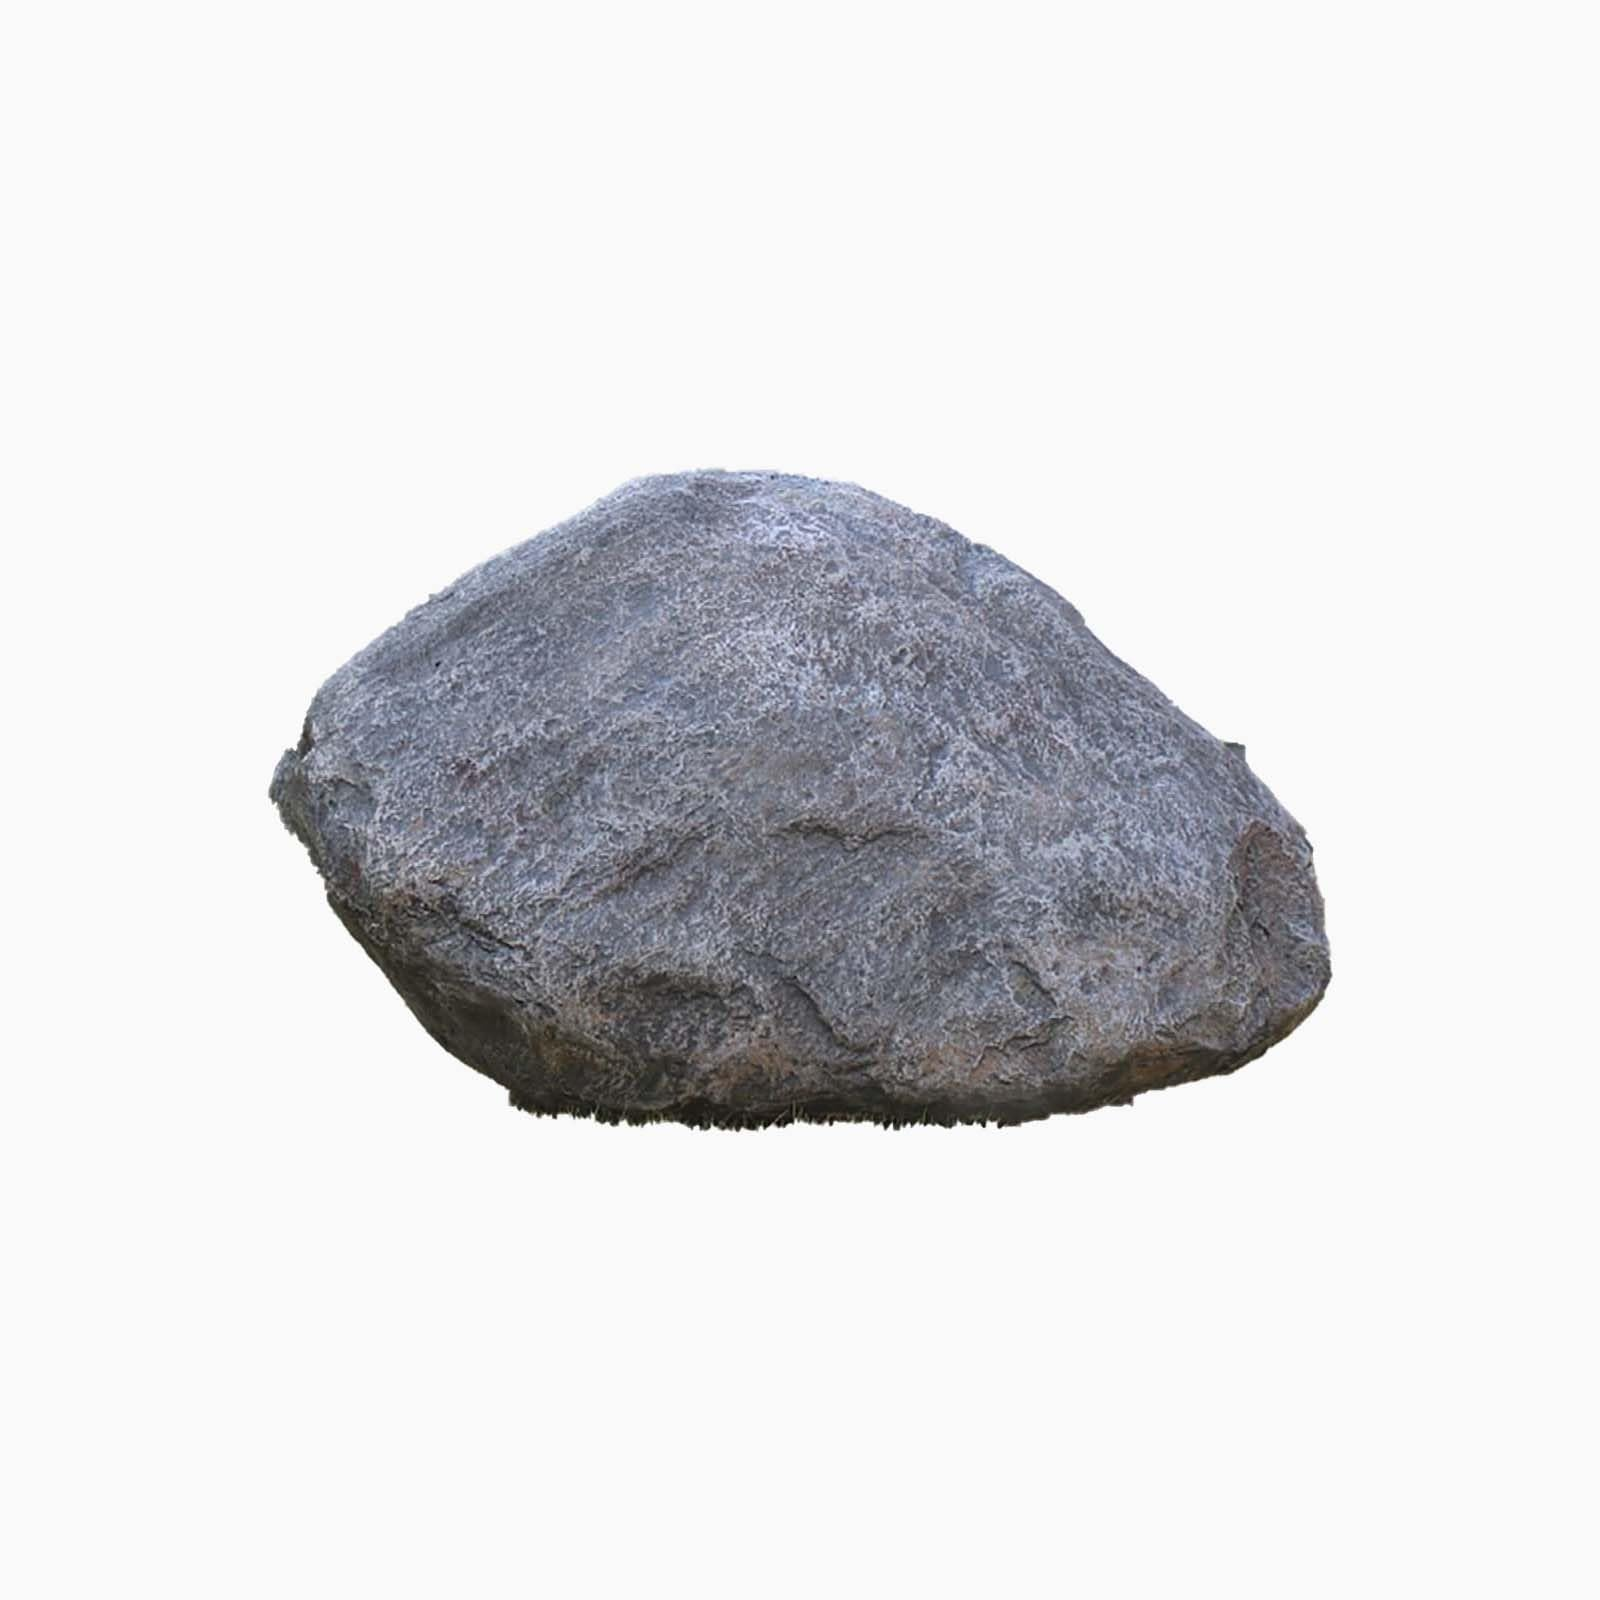
\includegraphics[width=2.4cm]{oui.jpg}
\end{minipage}\hfill
\begin{minipage}[c]{\dimexpr\textwidth-2.9cm\relax}
  {\fontsize{21}{24}\selectfont Pierre DUROCHER}\\[3pt]
  {\itshape Software Engineer -- Specialized in Cloud Architecture and Distributed Systems}\\[6pt]
  \begin{minipage}[t]{0.56\linewidth}\small
    Paris, France\\
    \href{mailto:p.durocher@email.com}{p.durocher@email.com}
  \end{minipage}\hfill
  \begin{minipage}[t]{0.40\linewidth}\small\raggedleft
    Tel.~: +33 6 66 66 66 66\\
    \href{https://linkedin.com/in/pierre-durocher/}{linkedin.com/in/pierre-durocher/}\\
    Driving licence
  \end{minipage}
\end{minipage}

\vspace{6pt}
{\noindent\color{accent}\rule{\textwidth}{1pt}}

% ---------- BODY ----------
\columnratio{0.655}
\setlength{\columnsep}{20pt}
\begin{paracol}{2}

% ===== LEFT COLUMN =====
\cvsection{Professional Summary}
\vspace{5pt}
{\small Software engineer specialised in cloud architecture and distributed systems, currently leading microservices development at TechCorp SAS. Background spanning backend engineering, DevOps and large-scale system design, with a focus on performance, reliability and team leadership.\par}

\cvsection{Education}

\cventry{École Polytechnique, Paris}
  {Master's in Computer Science • Paris, France}
  {Sept. 2019 -- June 2021}
{\footnotesize\itshape Specialisation in Distributed Systems and Cloud Computing. GPA: 3.8/4.0. Thesis on microservices architecture optimization.\par}

\cventry{Université Paris-Tech}
  {Bachelor's in Engineering • Paris, France}
  {Sept. 2016 -- June 2019}
{\footnotesize\itshape Major in Software Engineering. Recipient of the Academic Excellence Scholarship. Completed internship at leading tech company.\par}

\cvsection{Professional Experience}

\cventry{Senior Software Engineer}
  {TechCorp SAS • France}
  {March 2023 -- ongoing}
{\footnotesize\itshape Led development of microservices architecture serving 2M+ users. Mentored 3 junior engineers. Reduced API latency by 35\% through optimization work.\par\vspace{3.5pt}
Skills: Kubernetes · gRPC · performance tuning · team leadership.\par}

\cventry{Software Engineer}
  {CloudSys GmbH}
  {July 2021 -- Feb. 2023}
{\footnotesize\itshape Developed backend services using Go and Python. Implemented CI/CD pipelines with GitLab CI. Contributed to 4 major product releases.\par\vspace{3.5pt}
Skills: Go · PostgreSQL · cloud DevOps · Agile methodologies.\par}

\cventry{Software Engineering Intern}
  {Innovate Labs}
  {June 2020 -- Aug. 2020}
{\footnotesize\itshape Developed features for internal data platform. Fixed 15+ bugs reported by QA team. Earned full-time offer upon graduation.\par\vspace{3.5pt}
Skills acquired: Java · software testing · professional development.\par}

\cvsection{Projects}
\vspace{5pt}
{\footnotesize
\textbf{Distributed Task Scheduler} -- Academic - Python, Docker, Kubernetes\par
\itshape Team of 4 over 6 months. High-performance task scheduler for distributed computing. Optimised throughput by 40\% through load balancing algorithms. Containerised with Docker and orchestrated using Kubernetes.\upshape\par\vspace{3pt}
\textbf{Real-time Data Pipeline} -- Academic - Kafka, Spark, Python\par
\itshape Lead developer, team of 3, over 4 months. Real-time data processing pipeline handling 500K events per second, with fault tolerance and auto-scaling mechanisms.\upshape\par\vspace{3pt}
\textbf{Compiler Optimization Project} -- Academic - C++, LLVM\par
\itshape Solo project over 3 months. Compiler optimisations for functional languages, achieving a 25\% improvement in code generation efficiency.\upshape\par\vspace{3pt}
\textbf{Cloud Cost Analytics Dashboard} -- Academic - React, Node.js, PostgreSQL\par
\itshape Full-stack developer, team of 2, over 5 months. Analytics platform for monitoring AWS costs in real time, helping reduce cloud spending by 20\%.\upshape\par}

\switchcolumn

% ===== RIGHT COLUMN =====
\cvsection{Areas of Expertise}
\vspace{5pt}
\cvdomain{Skills}{%
Problem-solving · System design · Leadership · Attention to detail · Communication}

\vspace{7pt}

\cvdomain{Tools}{%
Docker · Kubernetes · AWS · Git · GitLab CI · Jenkins · Linux/Unix}

\vspace{7pt}

\cvdomain{Programming}{%
Python · Go · Java · C++ · PostgreSQL · MongoDB · Redis · SQL optimisation · Microservices architecture · RESTful APIs · gRPC}

\vspace{7pt}

\cvdomain{Currently Learning}{%
Rust · Machine Learning basics · WebAssembly}

\cvsection{Languages}
\vspace{5pt}
{\small
\cvlang{French}{\lin{Native speaker}}
\cvlang{English}{\lin{C1} -- TOEIC 920/990}
\cvlang{German}{\lin{B1}}}

\cvsection{Interests}
\vspace{5pt}
{\small
\textbf{Open Source}~: Active contributor to Kubernetes and Prometheus projects.\par\vspace{3.5pt}
\textbf{Technology Blogging}~: Writes technical articles on distributed systems and cloud architecture.\par\vspace{3.5pt}
\textbf{Rock Climbing}~: Weekend climber, completed several outdoor climbing routes.\par}

\end{paracol}

\end{document}
